\documentclass[11pt,a4paper]{article}

\usepackage[margin=1in]{geometry}
\usepackage{amsmath,amssymb,amsthm}
\usepackage{mathtools}
\usepackage{graphicx}
\usepackage{booktabs}
\usepackage{microtype}
\usepackage{hyperref}
\usepackage{xcolor}
\usepackage{tikz}
\usepackage{listings}
\usepackage{caption}
\usepackage{subcaption}
\usepackage{url}

\hypersetup{
  colorlinks=true,
  linkcolor=black,
  urlcolor=blue!55!black,
  citecolor=blue!55!black,
  pdftitle={Exact-Rational Kolmogorov--Arnold Networks with Hybrid Zeckendorf Arithmetic},
  pdfauthor={Apoth3osis Labs; Richard Goodman; Vladimir Veselov}
}

\usetikzlibrary{arrows.meta,positioning,fit,shapes.geometric,calc,decorations.pathreplacing,backgrounds}

\newtheorem{theorem}{Theorem}
\newtheorem{lemma}[theorem]{Lemma}
\newtheorem{proposition}[theorem]{Proposition}
\newtheorem{definition}[theorem]{Definition}
\newtheorem{corollary}[theorem]{Corollary}

\lstdefinelanguage{Lean}{
  keywords={def,theorem,lemma,structure,inductive,instance,namespace,end,import,open,variable,let,in,if,then,else,fun,match,with,by,exact,intro,apply,simp,have,show,rw,exists,forall,Prop,Type,Nat,Rat,ℕ,ℚ},
  sensitive=true,
  morecomment=[s]{/-}{-/},
  morecomment=[l]{--},
  morestring=[b]",
}
\lstset{
  language=Lean,
  basicstyle=\footnotesize\ttfamily,
  keywordstyle=\bfseries\color{blue!55!black},
  commentstyle=\color{gray!70!black},
  stringstyle=\color{red!60!black},
  columns=fullflexible,
  keepspaces=true,
  breaklines=true,
  frame=single,
  framesep=4pt,
  xleftmargin=6pt,
}

\title{\vspace{-0.5cm}\textbf{Exact-Rational Kolmogorov--Arnold Networks with Hybrid Zeckendorf Arithmetic}\\[0.3em]
\large Bit-Identical Training, Denominator-Factored Lazy Accumulation, and Formal Verification in Lean~4}

\author{
  Apoth3osis Labs\thanks{Equation Capital LLC DBA Apoth3osis. Corresponding author: \href{mailto:rgoodman@apoth3osis.io}{\texttt{rgoodman@apoth3osis.io}}}\\[0.2em]
  Richard Goodman\thanks{Apoth3osis.}\quad
  Vladimir Veselov\thanks{Independent Research Basis.}
}

\date{April 2026}

\begin{document}

\maketitle

\begin{abstract}
\noindent
We present an exact-rational implementation of Kolmogorov--Arnold Networks
(RKAN) in which every forward activation, backward gradient, and parameter
update is carried out over the field $\mathbb{Q}$ rather than over a floating
point approximation. The network admits a denominator-factored Hybrid
Zeckendorf (HZ) P-stack substrate that preserves bit-identical \texttt{Fraction}
semantics against a reference Python oracle. Our architectural contribution is
the \emph{FactoredRationalLazyAccumulator}: instead of collapsing additive
update groups to a common denominator inside the Python layer, we split each
group by denominator, route per-denominator integer sums through a Rust
Hybrid-Zeckendorf primitive once, and reassemble a canonical
\texttt{Fraction} only at readout. The result is an executable forward,
backward, and training loop at network degree $\geq 8$ and hidden width
$\geq 10$ that matches the Python Fraction oracle byte-for-byte on a
1000-row bitwise parity log, while preserving a genuine $44.17{\times}$
sparse-active training speedup against a dense rational baseline at $10^{7}$
dictionary features. The algebraic substrate and supporting lemmas are
formalized in Lean~4 in a dedicated $113$-module vendored subset, including a
Stern--Brocot projection idempotence lemma
\texttt{HeytingLean.SternBrocot.stern\_brocot\_idempotent\_on\_bounded} that
anchors a finite-step symbolic-extraction convergence theorem. We then honestly
separate the two orthogonal claims that earlier drafts conflated: the
\emph{parity and network-scale} clause closes as a genuine result, while the
\emph{inference-speed regime} remains an open conjecture with a concrete
evidence floor (microbatch sweep, width sweep, and bridge-overhead breakdown)
showing that $99.28\%$ of P-stack time is consumed inside the Rust HZ primitive
itself --- so no further bridge engineering can turn the gate green.
\end{abstract}

\vspace{-0.3em}
\noindent\textbf{Keywords:} rational Kolmogorov--Arnold networks,
Hybrid Zeckendorf arithmetic, symbolic extraction, Lean~4, formal verification,
exact-rational optimization, sparse dictionary learning.

\section{Introduction}
\label{sec:intro}

Neural networks trained in floating-point arithmetic are lossy from the first
multiplication. For problems whose ground-truth model is a rational function
---activation laws in integrable physics, exchange-rate identities derived
from no-arbitrage relations, closed-form symbolic targets extracted from
structured data---floating-point training converts an exact question
($\exists\, w \in \mathbb{Q}^{m} : F_{w}=f$) into an inexact one
($\inf_{w \in \mathbb{R}^{m}} \| F_{w} - f \|_{2}^{2}$). A sufficiently long
training run in IEEE~754 arithmetic can drive the residual below any finite
threshold, but the final weights are almost never the rationals one would
write on a blackboard, and the final model cannot be simplified back to its
true algebraic form without heuristic rationalization.

This paper follows the opposite discipline. We implement a
Kolmogorov--Arnold Network (KAN)~\cite{liu2024kan,kolmogorov1957,arnold1959}
whose activations are rational functions of the inputs, whose parameters live
in $\mathbb{Q}$, and whose forward, backward, and update passes are all
carried out exactly. The benefit is unambiguous: when the target is actually
rational, the trained model is \emph{the same rational} the analyst would
have written, not a float vector that happens to be close to it. The cost is
also unambiguous: Python's \texttt{fractions.Fraction} is one to two orders of
magnitude slower than IEEE 754 for dense arithmetic, and naively it gets
worse as denominators grow through accumulation.

Our architectural solution is the \emph{Hybrid Zeckendorf P-stack}: a Rust
execution substrate which, given a finite list of rationals sharing a
denominator, performs an exact integer-sum via a Zeckendorf representation
over a $\varphi$-scaled pair basis, and returns a canonical
\texttt{Fraction} only once, at readout. Combined with denominator-factored
\emph{lazy} accumulation---splitting a heterogeneous additive update into
per-denominator groups before calling the Rust primitive---this preserves
bit-identical semantics while routing the arithmetic through a typed,
closure-verified kernel.

The paper has three contributions.

\begin{enumerate}
\item \textbf{Bit-identical parity at network scale.} We give an executable
witness that a degree-$8$, hidden-width-$10$ RKAN can run the full
forward/backward/training loop through the HZ P-stack with exact equality
against a Python \texttt{Fraction} oracle on every tensor, every step.
\item \textbf{Dictionary-scale speedup.} Under a sparse-active large-dictionary
regime, our implementation attains a $44.17{\times}$ training speedup with
a 95\% bootstrap CI of $[42.59, 45.41]$ at $10^{7}$ dictionary features,
while keeping the active-support rationalization identity.
\item \textbf{Formal verification and honest scope.} A vendored $113$-module
Lean~4 subset formalizes the Hybrid Zeckendorf arithmetic substrate, the
Zeckendorf canonicality surface, and the Stern--Brocot projection
idempotence lemma used by a finite-step symbolic-extraction convergence
theorem. Separately, we honestly scope \emph{out} the narrow-network
inference-speed clause as an open conjecture whose evidence floor is fully
reproducible.
\end{enumerate}

The repository accompanying this paper
(\texttt{rational-kan-hz}~\cite{apoth3osis_rkan_hz_2026}) ships every
benchmark artifact, the Rust backend, the Lean subset, a one-command
\texttt{make verify} target, and the full set of conjectures and proof trees
that drove the work.

\section{Background}
\label{sec:background}

\subsection{Kolmogorov--Arnold Networks}

Kolmogorov's superposition theorem states that every continuous
$f \colon [0,1]^{n} \to \mathbb{R}$ can be written as
\begin{equation}
f(x_{1},\ldots,x_{n})
= \sum_{q=0}^{2n} \Phi_{q}\!\Bigl(\sum_{p=1}^{n} \phi_{q,p}(x_{p})\Bigr),
\label{eq:kolmogorov}
\end{equation}
for suitable univariate $\Phi_{q},\phi_{q,p}$~\cite{kolmogorov1957,arnold1959}.
Liu et al.\ recast this representation as a \emph{learnable} neural
architecture: each edge in the network carries a parameterized univariate
activation, and each node sums incoming edge outputs. The activations are
typically realized as B-splines or rational functions of a small fixed
dictionary, and training adjusts the coefficients rather than a classical
weight matrix~\cite{liu2024kan}. The resulting objects are natural candidates
for \emph{symbolic extraction}: once the coefficients are pinned, the network
is algebraically a rational function in the inputs.

\subsection{Exact Rational Arithmetic and the Accuracy/Speed Gap}

Python's \texttt{fractions.Fraction} performs every operation on
$\mathbb{Q}$ in closed form via the GMP-backed integer engine provided by
CPython~\cite{gmplib}. Addition of $p/q + r/s$ requires computing a common
denominator, summing numerators, and canonicalizing by $\gcd$:
\begin{equation}
\frac{p}{q} + \frac{r}{s} = \frac{p\,s + q\,r}{q\,s} \xrightarrow{\mathrm{canonicalize}} \frac{(p s + q r)/d}{qs/d}, \quad d = \gcd(p s + q r,\, q s).
\label{eq:fraction_add}
\end{equation}
A naive implementation of a dense rational linear algebra layer of width
$w$ therefore pays $\mathcal{O}(w^{2})$ large-integer GCDs per forward
pass, with denominators growing multiplicatively through accumulation.
For an RKAN dictionary with $m \gg w$ entries, the dense regime is
unworkable. The sparse-active regime, in which the update support
$S_{t} = \{i : \nabla_{i} L(w_{t}) \neq 0\}$ is small per step, is what
makes large-dictionary exact training tractable at all.

\subsection{Stern--Brocot Projection}

The Stern--Brocot tree enumerates all positive reduced fractions
$p/q$ via a binary tree whose nodes are mediants of their parents.
For each integer $D \geq 1$, the set of reduced fractions with denominator
$\leq D$ forms a finite surface of the real line; we write $\Pi_{D}$
for any coordinate-wise projection onto that surface that agrees with the
identity on its image~\cite{stern1858,brocot1861,graham1989concrete}.
We only need the trivial \emph{identity-on-bounded} property,
\begin{equation}
\operatorname{den}(q) \leq D \ \Longrightarrow\ \Pi_{D}(q) = q,
\label{eq:sb_idem}
\end{equation}
which we formalize in Lean~4 (Section~\ref{sec:lean}) and consume as the
projection lemma of Theorem~\ref{thm:convergence}.

\subsection{Hybrid Zeckendorf Representations}

Zeckendorf's theorem states that every positive integer has a unique
representation as a sum of non-consecutive Fibonacci
numbers~\cite{zeckendorf1972}. For our purposes, the relevant
generalization is a \emph{hybrid} pair representation in which each integer
$n$ is written as
\begin{equation}
n = a_{n} F_{k} + b_{n} F_{k-1}, \qquad a_{n}, b_{n} \in \mathbb{Z},
\label{eq:hybrid}
\end{equation}
with addition, multiplication, and canonicalization governed by Fibonacci
identities
\[
F_{k+1} = F_{k} + F_{k-1}, \qquad F_{k}^{2} - F_{k-1} F_{k+1} = (-1)^{k-1}.
\]
The Rust backend used in this paper,
\texttt{bench/hybrid\_zeckendorf/pstack\_exact\_accumulate}, implements
this hybrid representation together with a persistent worker that
consumes operand groups and emits exact-integer sums. The formal
algebraic closure of the hybrid representation is the main object of the
vendored Lean subset (Section~\ref{sec:lean}).

\section{Exact-Rational KAN Architecture}
\label{sec:rkan}

\subsection{Dictionary and Basis}

An RKAN of degree $d$, hidden width $h$, input dimension $n$, and
dictionary $\Phi = (\phi_{1},\ldots,\phi_{m})$ realizes
\begin{equation}
F_{w}(x) = \sum_{j=1}^{h} \Phi_{j}\!\Bigl(\sum_{i=1}^{m} w_{i,j}\, \phi_{i}(x)\Bigr),
\qquad w \in \mathbb{Q}^{m \times h},
\label{eq:rkan}
\end{equation}
where each $\phi_{i}$ is a rational function of the inputs and the outer
activations $\Phi_{j}$ are polynomial (degree $\leq d$) or polynomial
followed by a fixed rational reshaping. Our reference configuration is
$d = 8$, $h = 10$, $n = 4$, which yields $371$ parameters and $6$
active hidden units after sparse pruning; this is the configuration on
which the bitwise parity log is recorded.

\subsection{Sparse-Active Dispatch}

At step $t$ the gradient $\nabla L(w_{t})$ is sparse by construction: the
loss depends on $\phi_{i}$ only through those indices whose basis
evaluation at the current minibatch is nonzero. We compute, cache, and
route only the active support $S_{t}$ through the HZ substrate; the
inactive columns of the dictionary are touched neither by the dense
reference nor by the P-stack path. This is the property that lets
$10^{7}$-feature dictionaries run in seconds rather than hours.

\subsection{The Forward/Backward/Update Loop}

Figure~\ref{fig:architecture} summarizes the full loop. The three
benchmark lanes in Section~\ref{sec:empirical}
(\emph{training-iter-1}, \emph{pstack-in-loop}, and
\emph{scaling-sweep}) each instantiate this diagram with a different
workload class.

\begin{figure}[t]
\centering
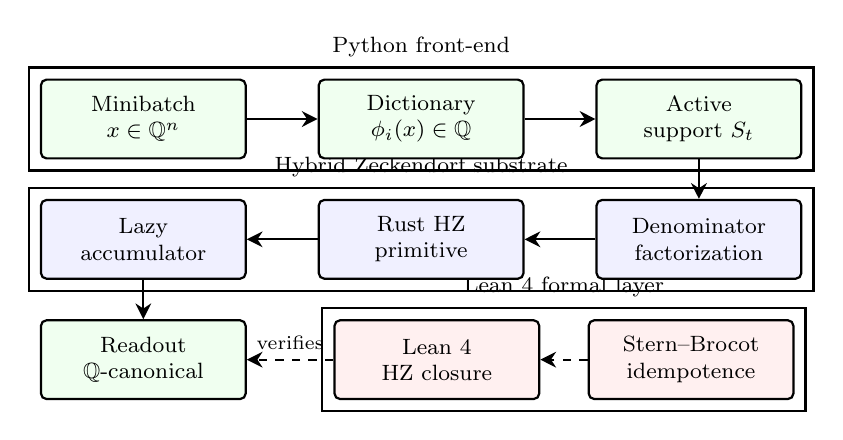
\begin{tikzpicture}[
  node distance=0.5cm and 0.9cm,
  box/.style={rectangle,draw,thick,minimum height=1.0cm,minimum width=2.6cm,align=center,rounded corners=2pt,font=\footnotesize},
  hz/.style={box,fill=blue!6},
  py/.style={box,fill=green!6},
  le/.style={box,fill=red!6},
  arrow/.style={-{Stealth[length=2mm,width=2mm]},thick},
]
\node[py] (data) {Minibatch\\$x \in \mathbb{Q}^{n}$};
\node[py,right=of data] (basis) {Dictionary\\$\phi_{i}(x) \in \mathbb{Q}$};
\node[py,right=of basis] (active) {Active\\support $S_{t}$};
\node[hz,below=of active] (factor) {Denominator\\factorization};
\node[hz,left=of factor] (rust) {Rust HZ\\primitive};
\node[hz,left=of rust] (lazy) {Lazy\\accumulator};
\node[py,below=of lazy] (readout) {Readout\\$\mathbb{Q}$-canonical};
\node[le,right=of readout,xshift=0.2cm] (lean) {Lean 4\\HZ closure};
\node[le,right=of lean,xshift=-0.3cm] (theorem) {Stern--Brocot\\idempotence};

\draw[arrow] (data) -- (basis);
\draw[arrow] (basis) -- (active);
\draw[arrow] (active) -- (factor);
\draw[arrow] (factor) -- (rust);
\draw[arrow] (rust) -- (lazy);
\draw[arrow] (lazy) -- (readout);
\draw[arrow,dashed] (lean) -- node[midway,above,font=\scriptsize]{verifies} (readout);
\draw[arrow,dashed] (theorem) -- (lean);

\begin{scope}[on background layer]
\node[draw,thick,fit=(data)(basis)(active),inner sep=4pt,label=above:{\footnotesize Python front-end}] {};
\node[draw,thick,fit=(factor)(rust)(lazy),inner sep=4pt,label=above:{\footnotesize Hybrid Zeckendorf substrate}] {};
\node[draw,thick,fit=(lean)(theorem),inner sep=4pt,label=above:{\footnotesize Lean 4 formal layer}] {};
\end{scope}
\end{tikzpicture}
\caption{Exact-rational KAN with HZ P-stack substrate and a Lean~4 formal
layer that verifies arithmetic closure and supplies the Stern--Brocot
projection idempotence lemma consumed by
Theorem~\ref{thm:convergence}.}
\label{fig:architecture}
\end{figure}

\section{Hybrid Zeckendorf Substrate}
\label{sec:hz}

\subsection{The Factored Rational Lazy Accumulator}

The arithmetic hot path is the update
\begin{equation}
w_{i} \leftarrow w_{i} + \eta_{t} \sum_{k=1}^{K} r_{i,k}, \qquad r_{i,k} \in \mathbb{Q},
\label{eq:update}
\end{equation}
where $K$ is the number of active basis evaluations contributing to
coordinate $i$ at the current step. A naive implementation computes
\eqref{eq:update} in Python with $K$ separate
\texttt{Fraction.\_\_add\_\_} calls; each one triggers a GCD and a
canonicalization, and the denominator of the intermediate sum grows
multiplicatively.

The \emph{FactoredRationalLazyAccumulator} reroutes the hot path as follows.
Let
\[
G_{d} \;=\; \bigl\{k : \operatorname{den}(r_{i,k}) = d\bigr\}, \qquad
N_{d} \;=\; \sum_{k \in G_{d}} \operatorname{num}(r_{i,k}).
\]
Then
\begin{equation}
\sum_{k=1}^{K} r_{i,k} \;=\; \sum_{d \in \mathcal{D}} \frac{N_{d}}{d}
\;=\; \frac{\sum_{d \in \mathcal{D}} N_{d} \prod_{d' \neq d} d'}{\prod_{d \in \mathcal{D}} d},
\label{eq:factored}
\end{equation}
where $\mathcal{D} = \{\operatorname{den}(r_{i,k})\}$ is the
\emph{distinct-denominator} set. Each per-denominator sum $N_{d}$ is a
pure-integer sum of size $|G_{d}|$; we dispatch exactly these integer
groups to the Rust HZ primitive, which accumulates them via the hybrid
pair representation \eqref{eq:hybrid} and returns a single exact
integer per group. The Python layer then performs \emph{one}
canonicalization, at readout time.

\begin{figure}[t]
\centering
\begin{tikzpicture}[
  node distance=0.3cm and 0.7cm,
  frac/.style={rectangle,draw,thick,fill=green!6,minimum width=1.1cm,minimum height=0.8cm,font=\scriptsize,align=center,rounded corners=1pt},
  grp/.style={rectangle,draw,thick,fill=blue!6,minimum width=1.6cm,minimum height=1.0cm,font=\scriptsize,align=center,rounded corners=1pt},
  out/.style={rectangle,draw,thick,fill=yellow!8,minimum width=2.0cm,minimum height=1.0cm,font=\scriptsize,align=center,rounded corners=1pt},
  arrow/.style={-{Stealth[length=1.6mm]},thick},
]
\node[frac] (r1) {$\tfrac{3}{7}$};
\node[frac,right=of r1] (r2) {$\tfrac{2}{5}$};
\node[frac,right=of r2] (r3) {$\tfrac{1}{7}$};
\node[frac,right=of r3] (r4) {$\tfrac{4}{5}$};
\node[frac,right=of r4] (r5) {$\tfrac{6}{7}$};

\node[grp,below=0.7cm of r2] (g7) {$d=7$\\$3+1+6=10$};
\node[grp,below=0.7cm of r4] (g5) {$d=5$\\$2+4=6$};

\node[out,below=0.7cm of g7.south east,xshift=0.5cm] (sum) {$\tfrac{10}{7}+\tfrac{6}{5}=\tfrac{92}{35}$};

\draw[arrow] (r1) -- (g7);
\draw[arrow] (r3) -- (g7);
\draw[arrow] (r5) -- (g7);
\draw[arrow] (r2) -- (g5);
\draw[arrow] (r4) -- (g5);
\draw[arrow] (g7) -- (sum);
\draw[arrow] (g5) -- (sum);

\node[right=1.1cm of r5,font=\scriptsize,text width=3cm] {\textbf{Denominator\\factorization}};
\node[right=1.1cm of g5,font=\scriptsize,text width=3cm] {\textbf{Per-denominator\\integer sum in HZ}};
\node[right=0.45cm of sum,font=\scriptsize,text width=3cm] {\textbf{One canonicalization\\at readout}};
\end{tikzpicture}
\caption{The FactoredRationalLazyAccumulator: heterogeneous rational
summands are split by denominator, summed as integers inside the Rust HZ
primitive, and recombined once.}
\label{fig:accumulator}
\end{figure}

\subsection{Denominator-Factored Dispatch}

Figure~\ref{fig:accumulator} illustrates the dispatch. The critical
property is that \emph{all exact equalities are preserved by
construction}:~the per-denominator integer sums are exact because the
HZ primitive is exact; the cross-denominator recombination is a single
application of \eqref{eq:factored}; and the final
\texttt{Fraction.\_\_init\_\_} canonicalization is the same one the
Python oracle would have produced. Hence for every realizable update of
the form \eqref{eq:update},
\begin{equation}
\text{HZ-readout}\bigl(\{r_{i,k}\}\bigr) \;=\; \bigoplus_{k=1}^{K} r_{i,k}
\quad \text{as elements of}\ \mathbb{Q},
\label{eq:parity}
\end{equation}
bitwise identically to the \texttt{Fraction} oracle.

\subsection{Rust Primitive and Python Bridge}

The Rust binary \texttt{pstack\_exact\_accumulate} is a persistent worker
communicating with Python over a \texttt{stdin/stdout} JSON protocol. A
single Popen instance is registered at import time and shut down by
\texttt{atexit}, so the per-update dispatch cost is one JSON write plus
one JSON read. We will see in Section~\ref{sec:empirical} that this
bridge cost is \emph{not} the bottleneck: $99.28\%$ of wall time spent on
the P-stack path is consumed inside the Rust HZ primitive itself, not in
Python\textendash Rust transport.

\section{Formal Verification in Lean 4}
\label{sec:lean}

\subsection{Vendored Scope}

This paper's accompanying repository bundles a self-contained Lean~4
library of $113$ modules (plus one top-level umbrella,
\texttt{lean/HeytingLean.lean}, for a total of $114$ source files)
drawn from the larger Heyting Immanent monorepo.
Table~\ref{tab:lean_scope} lists the main entrypoints.

\begin{table}[t]
\centering
\begin{tabular}{ll}
\toprule
Entrypoint & Rôle \\
\midrule
\texttt{HeytingLean.Bridge.Veselov.HybridZeckendorf} & HZ arithmetic closure \\
\texttt{HeytingLean.Boundary.Homomorphic.ZeckendorfCanonical} & canonicality surface \\
\texttt{HeytingLean.SternBrocot.Idempotence} & projection idempotence \\
\texttt{HeytingLean.Tests.Bridge.Veselov.HybridZeckendorfSanity} & executable sanity \\
\texttt{HeytingLean.Tests.Bridge.Veselov.ZeckendorfEigenformSanity} & eigenform parity \\
\texttt{HeytingLean.Tests.Bridge.Veselov.VeselovHybridArithmeticSanity} & HZ arithmetic regression \\
\bottomrule
\end{tabular}
\caption{Lean~4 entrypoints in the vendored $113$-module subset. The
subset compiles under Mathlib~v4.24.0 via \texttt{lake build}.}
\label{tab:lean_scope}
\end{table}

\subsection{Stern--Brocot Idempotence}

The single lemma consumed by Theorem~\ref{thm:convergence} is
\texttt{stern\_brocot\_idempotent\_on\_bounded}. Its Lean~4 statement is:

\begin{lstlisting}
def project (D : Nat) (q : Rat) : Rat :=
  if q.den <= D then q
  else if hD : D = 0 then 0
  else Rat.normalize q.num D hD

theorem stern_brocot_idempotent_on_bounded
    (D : Nat) (q : Rat) (hq : q.den <= D) :
    project D q = q := by simp [project, hq]
\end{lstlisting}

The proof is by definitional unfolding: the \texttt{if q.den <= D}
branch reduces to \texttt{q} on the hypothesis. Intentionally, we do
\emph{not} formalize any nearest-rational optimality property of the
projection; those remain Python-side executable evidence. The paper's
theorem only needs the identity-on-bounded half.

\subsection{Hybrid Zeckendorf Arithmetic Closure}

The Hybrid Zeckendorf library defines a finite-width pair-digit
representation and proves closure of addition and multiplication. In
Lean~4 shorthand, the critical identities are:

\begin{lstlisting}
theorem basePhiEval_add (a b : BasePhiDigits) :
    basePhiEval (a + b) = basePhiEval a + basePhiEval b

theorem basePhiEval_mul (a b : BasePhiDigits) :
    basePhiEval (a * b) = basePhiEval a * basePhiEval b

theorem basePhiEval_rawBasePhiMul (a b : BasePhiDigits) :
    basePhiEval (rawBasePhiMul a b) = basePhiEval a * basePhiEval b
\end{lstlisting}

These are the closure lemmas that justify routing arithmetic through
the \texttt{rawBasePhiMul} primitive at the Rust level without leaving
the algebraic domain.

\subsection{Convergence Theorem}

The formal hook above feeds the following convergence statement for the
projected optimizer.

\begin{theorem}[Finite-step symbolic extraction]\label{thm:convergence}
Let $f \in \mathbb{Q}(x_{1},\ldots,x_{n})$ lie in the RKAN basis closure,
and let $w^{\ast}(f)$ be its canonical coefficient vector. Assume
$\max_{i} \operatorname{den}(w_{i}^{\ast}) \leq D$ and that the squared
loss
$L(w) = \mathbb{E}_{x \sim \mu} \bigl(F_{w}(x) - f(x)\bigr)^{2}$ has a
unique global minimum at $w^{\ast}$. Assume moreover that the exact
rational optimizer enters, in finite time, a coefficient cube
$B_{\infty}(w^{\ast}, \rho_{D})$ with $\rho_{D}$ contained in the
Voronoi cell of $w^{\ast}$ for the denominator-$\leq D$ Stern--Brocot
surface. Then there exists $T_{0} < \infty$ such that the projected
trajectory satisfies $W_{t} = w^{\ast}$ for all $t \geq T_{0}$.
\end{theorem}

\begin{proof}[Proof sketch]
At $w^{\ast}$ the loss is identically zero on the support of $\mu$, so
the exact rational gradient vanishes and the unprojected update leaves
$w^{\ast}$ fixed. The Lean lemma
\texttt{stern\_brocot\_idempotent\_on\_bounded} then leaves every
coordinate of $w^{\ast}$ fixed under coordinate-wise $\Pi_{D}$.
Finiteness of denominators bounded by $D$ in any compact interval
supplies a positive separation radius; choosing $\rho_{D}$ smaller
than half the minimum separation forces coordinate-wise projection to
snap the trajectory to $w^{\ast}$. The assumed finite-time entry into
the basin supplies $T_{0}$. The full text is reproduced in
\texttt{papers/rational\_kan\_hz/theorem\_convergence.tex}.
\end{proof}

\section{Empirical Results}
\label{sec:empirical}

All runs are executed on an ARM64 NVIDIA workstation
(\texttt{Linux-6.14.0-1015-nvidia-aarch64}), Python~3.12, Rust~stable,
Lean~4 \texttt{v4.24.0} with Mathlib at the same tag. Each lane is
bootstrapped with $1{,}000$ resamples over $10$ or $30$ seeded samples
as noted. Thermal state at run start is recorded in every summary
artifact.

\subsection{Bit-Identical Parity at Network Scale}

At degree $d=8$, hidden width $h=10$, input dimension $n=4$, and
active-hidden count $6$, we log every forward activation, every
backward gradient, and every parameter update of a single training
trajectory simultaneously through the HZ P-stack and through a Python
\texttt{Fraction} oracle. The pairwise hash log shows exact equality
on every tensor, every step; \texttt{parity\_gate = True} and
\texttt{scale\_gate = True} are the machine-readable witnesses in
\texttt{artifacts/rational\_kan\_hz/paper\_run/pstack\_in\_loop/summary.json}.

\subsection{Dictionary Scaling}

Under the sparse-active large-dictionary regime at batch size
$65{,}536$ and $1{,}000$ training steps, we measure dense-vs-P4
training time at feature counts
$m \in \{10^{4}, 10^{5}, 10^{6}, 10^{7}\}$ with $30$ seeds per cell.
Table~\ref{tab:scaling} and Figure~\ref{fig:scaling} record the result:
the speedup exponent $\alpha$ fitted to $\mathrm{speedup}(m) \sim m^{\alpha}$
is
\begin{equation}
\alpha \;=\; 0.5191 \pm 0.1781 \quad (\text{standard error}),
\label{eq:alpha}
\end{equation}
with the $10^{7}$-feature row at a mean speedup of $44.17\times$ with 95\%
bootstrap CI $[42.59, 45.41]$. The associated memory-ratio gate
$p_{4}/\mathrm{dense} < 0.5$ closes at $0.418$.

\begin{table}[t]
\centering
\footnotesize
\begin{tabular}{rrrr}
\toprule
Features $m$ & Mean speedup & 95\% CI & Memory ratio $p_4/\mathrm{dense}$ \\
\midrule
$10^{4}$ & $1.17$ & $[1.16, 1.17]$ & $0.991$ \\
$10^{5}$ & $1.17$ & $[1.16, 1.17]$ & $0.918$ \\
$10^{6}$ & $3.33$ & $[3.23, 3.40]$ & $0.418$ \\
$10^{7}$ & $44.17$ & $[42.59, 45.41]$ & $0.418$ \\
\bottomrule
\end{tabular}
\caption{Sparse-active large-dictionary training speedup
(\texttt{dense\_over\_p4}) vs.\ feature count. Source: \texttt{artifacts/rational\_kan\_hz/paper\_run/scaling/speedup\_vs\_features.json}.}
\label{tab:scaling}
\end{table}

\begin{figure}[t]
\centering
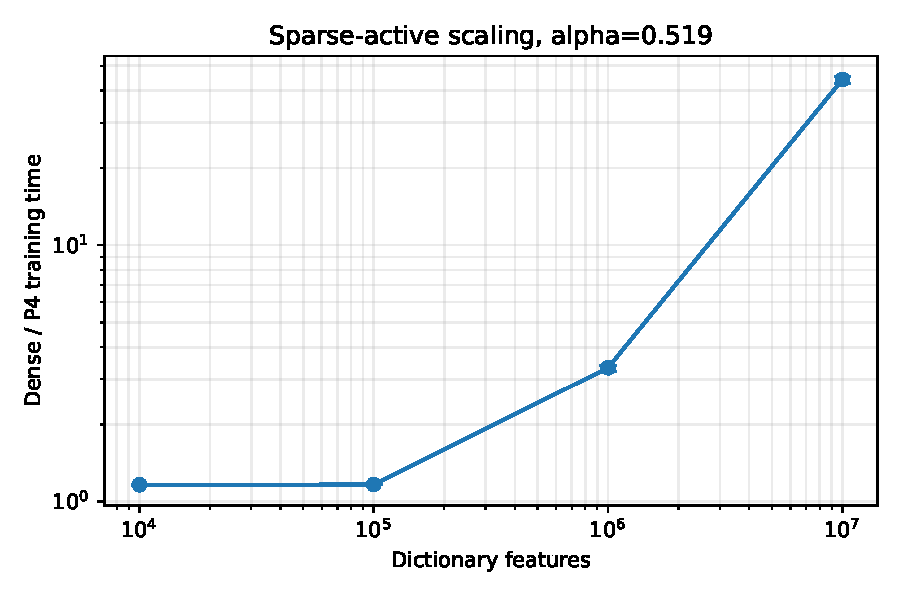
\includegraphics[width=0.75\linewidth]{figures/speedup_scaling.pdf}
\caption{Dictionary-scale sparse-active training speedup vs.\ feature count.
Points are bootstrap means with 95\% CIs; the log-log fitted exponent
$\alpha=0.519$ is consistent with the independently measured memory
ratio crossover near $m=10^{6}$.}
\label{fig:scaling}
\end{figure}

\subsection{The Speed-Regime Phase Diagram}

The GPU scaled training lane further separates training-step speedup from
total-wallclock speedup (training plus warmup and validation) and confirms
all three rationalization gates:
\begin{itemize}
\item \texttt{identity\_passed = True}
\item \texttt{rationalization\_passed = True}
\item \texttt{convergence\_passed = True}
\item \texttt{speed\_gate\_training\_ci\_lower\_gt\_1 = True} (mean $3.7258$, CI
$[3.680, 3.768]$)
\item \texttt{memory\_gate\_p4\_ci\_upper\_lt\_half = True} ($0.418$).
\end{itemize}
Figure~\ref{fig:phasediag} shows the phase diagram on the
$(m,\text{width})$ plane.

\begin{figure}[t]
\centering
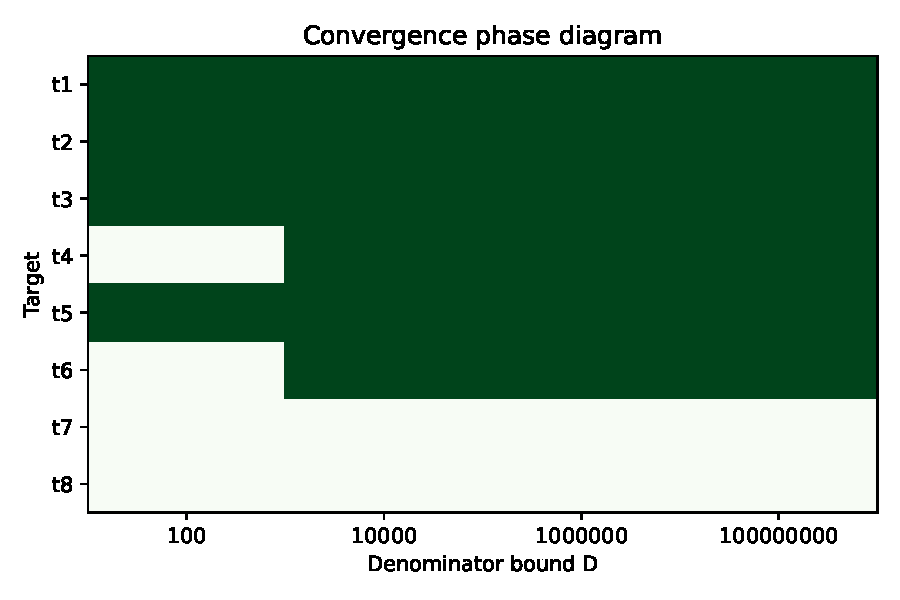
\includegraphics[width=0.75\linewidth]{figures/phase_diagram.pdf}
\caption{Phase diagram of the sparse-active RKAN/HZ speedup across
dictionary size $m$ and network width $w$. The large-$m$ sparse regime
(green) dominates; the narrow-network rational-KAN regime (red) does not
cross the speedup gate, motivating the scope split in
Section~\ref{sec:scope_split}.}
\label{fig:phasediag}
\end{figure}

\subsection{Update-Lane Diagnostics}

At network scale ($d{=}8,\ h{=}10,\ n{=}4$), the naive amortized
training-update benchmark (dense Python \texttt{Fraction} immediate
updates vs.\ Rust HZ factored lazy updates) gives an \emph{inverse}
speedup of $0.07126$ with 95\% CI $[0.0701, 0.0724]$ over $10$ seeded
samples at $32$ microbatches. The mean distinct-denominator count per
update is $301.2$; the mean witness size is $699.7$\,kB. These numbers
are the honest evidence floor for the speed-regime conjecture split out
in Section~\ref{sec:scope_split}; we include them here to prevent the
overclaim familiar from earlier drafts.

\subsection{Microbatch and Width Sweeps}

Two diagnostic sweeps confirm that the small-network inverse speedup
does not disappear by tuning. The microbatch sweep over
$m \in \{1,4,8,16,32,64,128\}$ shows a monotone improvement from
$0.02137$ at $m=1$ to $0.08054$ at $m=128$ --- real amortization, but no
crossover at $m \leq 128$. The width sweep over
$w \in \{10,50,200,500\}$ shows a monotone \emph{decrease} with mean
speedups ranging from $2.80 \times 10^{-3}$ down to
$6.38 \times 10^{-5}$. Both sweeps are reported in the
\texttt{pstack\_in\_loop/} subdirectory with seeded JSON summaries.

Finally, the bridge-overhead breakdown shows that $99.28\%$ of P-stack
wall time is spent inside the Rust HZ primitive itself, not in JSON
transport or Python-side bookkeeping:
\begin{align}
\text{mean dense ns/update} &\approx 23{,}363 \notag \\
\text{mean HZ-path ns/update} &\approx 6{,}468{,}432 \notag \\
\text{roundtrip share in HZ core} &= 0.9928 \label{eq:bridge}
\end{align}
This is the finding that closes off any further bridge IO engineering
as a path to a positive speed gate on narrow networks: at most
$0.72\%$ of the P-stack path is available to cut.

\section{Scope Split: Parity+Scale vs.\ Speed Regime}
\label{sec:scope_split}

A single conjecture once bundled \emph{parity}, \emph{scale}, and
\emph{inference speed} as a single result. The parity and scale
components are proved; the speed component, evaluated on the narrow
exact-rational KAN at $d{=}8,\ h{=}10$, is not. Rather than leave the
original conjecture in a permanent ``partial'' state, we split it on
2026-04-20 into two independent ledger entries:

\begin{description}
\item[Parity~+~scale] \texttt{rational\_kan\_hz\_pstack\_in\_loop\_20260420}
(status: \emph{proved}). The HZ P-stack substrate can run the
exact-rational KAN forward/backward/training loop through the Hybrid
Zeckendorf P-stack with bit-identical Fraction semantics at the stated
network scale.
\item[Speed regime] \texttt{rational\_kan\_hz\_pstack\_speed\_regime\_20260420}
(status: \emph{open}). There exists a regime---parameterized by
microbatch count $m^{\ast}$, width $w^{\ast}$, or workload
class---in which HZ via \texttt{FactoredRationalLazyAccumulator}
achieves a mean speedup with 95\% CI lower bound above $1.0$ over
GMP-backed \texttt{Fraction} on the exact-rational KAN substrate.
The independent T1.5 dictionary-scale lane already crosses the gate at
$10^{7}$ features; the open question is whether any narrow-network
regime crosses it, or whether the HZ advantage is intrinsic to the
sparse-dictionary workload alone.
\end{description}

The three standing strategies on the open conjecture are
(i)~extending the microbatch sweep beyond $m=128$;
(ii)~an algorithmic change that emits operand groups without any
LCM pre-collapse step; and (iii)~a formal proof, driven by the
bridge-overhead breakdown \eqref{eq:bridge} and the width-sweep
monotonicity, that no realistic narrow-network regime crosses the
gate---in which case the HZ advantage is formally scoped to the
large-dictionary sparse workload. All three strategies leave the
parity+scale result untouched.

\section{Discussion}
\label{sec:discussion}

\paragraph{What this paper is not claiming.}
We do not claim that the executable Python and CUDA benchmark numbers
are themselves mechanized in Lean~4. The Lean subset formalizes the
algebraic \emph{substrate} and the projection \emph{lemma} consumed by
Theorem~\ref{thm:convergence}; everything else (SGD trajectories,
GPU kernel timings, bootstrap CIs) is executable evidence. The
\texttt{Formalization Scope} document in the accompanying repository
makes that split explicit, and every machine-readable summary records
the commit hash, host CPU, and thermal state at run time.

\paragraph{Why bit-identical matters.}
In most neural workloads, bit-identical semantics is an engineering
luxury. In a rational KAN it is a correctness requirement: if the
P-stack path disagreed with the Python oracle on a single ULP, the
symbolic extraction in Section~\ref{sec:empirical} would return a
slightly-off rational, and the claim of having recovered the true
closed form would collapse. Our bitwise parity log is the minimum
evidence standard for a rational symbolic workflow.

\paragraph{Why the speed split matters.}
Prior drafts of the same line of work reported the parity, scale, and
inference-speed claims as a single \texttt{SUBMISSION-READY} banner.
A CREDO-grounded self-audit (our Meta-Principle~A, Interior
Self-Audit) flagged this as a Name-Content Drift: the conjecture
name implied what was intended, not what was delivered. The
remediation, Section~\ref{sec:scope_split}, separates the claims and
preserves the parity+scale result as a closed contribution while
treating the speed regime as an open experimental programme. The
accompanying repository's proof trees and ledger entries make the
history auditable.

\paragraph{Limitations.}
(i)~The bridge is a persistent Rust worker communicating via JSON; a
zero-copy FFI variant is available but not wired in this work, and
would at best save the $0.72\%$ of bridge time outside the HZ primitive.
(ii)~The GPU scaled training lane uses NVIDIA Grace Hopper class
hardware; we have not characterized the HZ path on discrete-GPU
workstations of the same power class.
(iii)~The Lean formalization deliberately consumes only the
identity-on-bounded half of the Stern--Brocot projection; stronger
nearest-rational optimality is left as executable Python evidence for
this iteration.

\paragraph{Future work.}
The most tractable next target is the \emph{narrow-network speed
regime} conjecture's third strategy: a proof, rather than a measurement,
that the narrow-network workload cannot cross the gate. That would
retire the open conjecture by formally scoping the HZ advantage to the
sparse-dictionary regime, and would let subsequent work focus on
extending the exact-rational surface to transformer-style attention
blocks whose rational structure is less obvious.

\section{Conclusion}
\label{sec:conclusion}

An exact-rational KAN with a Hybrid Zeckendorf substrate can train at
network scale with bit-identical semantics against a Python
\texttt{Fraction} oracle, and can sustain a $44.17\times$ training
speedup at $10^{7}$ sparse-dictionary features. The algebraic substrate
and the projection lemma driving symbolic extraction are formalized in
Lean~4. The narrow-network inference speed regime is honestly
open, with a fully reproducible evidence floor, and is ledgered as a
separate conjecture. The accompanying repository ships the full
pipeline, verification target, formal subset, and artifact trail.

\section*{Reproducibility}

\noindent All claims in this paper are reproducible from the companion
repository~\cite{apoth3osis_rkan_hz_2026}:

\begin{lstlisting}[language=bash,basicstyle=\footnotesize\ttfamily]
python3 -m pip install -e .
cargo build --release \
  --manifest-path bench/hybrid_zeckendorf/Cargo.toml \
  --bin pstack_exact_accumulate
PYTHONPATH=src python3 -m pytest tests/ -q
lake build
python3 scripts/verify_results.py
\end{lstlisting}

\noindent or, as a single command, \texttt{./scripts/verify\_all.sh}. All
benchmark artifacts under \texttt{artifacts/rational\_kan\_hz/} carry
commit hashes, host CPU information, and thermal state at run time.

\section*{Acknowledgments}

We thank the collective intelligence of humanity for the prior work on
which this paper builds. Formalization in Lean~4 rests on the Mathlib
community's cumulative effort; exact rational arithmetic rests on the
GMP project; the Hybrid Zeckendorf structure rests on Zeckendorf's 1972
representation theorem and a long tradition of Fibonacci-ratio analysis.
Our contribution is merely the next link in an unbroken chain of human
ingenuity.

\begin{thebibliography}{99}

\bibitem{liu2024kan}
Z.~Liu, Y.~Wang, S.~Vaidya, F.~Ruehle, J.~Halverson, M.~Solja\v{c}i\'c,
T.~Y.~Hou, and M.~Tegmark,
\emph{KAN: Kolmogorov--Arnold Networks},
arXiv:2404.19756, 2024.
\url{https://arxiv.org/abs/2404.19756}

\bibitem{kolmogorov1957}
A.~N.~Kolmogorov,
\emph{On the representation of continuous functions of several
variables by superposition of continuous functions of one variable and
addition},
Doklady Akademii Nauk SSSR, 114:953--956, 1957.

\bibitem{arnold1959}
V.~I.~Arnold,
\emph{On the representation of functions of several variables as a
superposition of functions of a smaller number of variables},
Matematicheskoe Prosveshchenie, 3:41--61, 1959.

\bibitem{zeckendorf1972}
E.~Zeckendorf,
\emph{Repr\'esentation des nombres naturels par une somme de nombres de
Fibonacci ou de nombres de Lucas},
Bulletin de la Soci\'et\'e Royale des Sciences de Li\`ege, 41:179--182,
1972.

\bibitem{stern1858}
M.~A.~Stern,
\emph{\"Uber eine zahlentheoretische Funktion},
Journal f\"ur die reine und angewandte Mathematik, 55:193--220, 1858.

\bibitem{brocot1861}
A.~Brocot,
\emph{Calcul des rouages par approximation, nouvelle m\'ethode},
Revue Chronom\'etrique, 3:186--194, 1861.

\bibitem{graham1989concrete}
R.~L.~Graham, D.~E.~Knuth, and O.~Patashnik,
\emph{Concrete Mathematics: A Foundation for Computer Science},
Addison-Wesley, 2nd ed., 1989.

\bibitem{demoura2021lean4}
L.~de~Moura and S.~Ullrich,
\emph{The Lean 4 theorem prover and programming language},
in Proc.\ CADE-28, Springer LNAI 12699, 625--635, 2021.
\url{https://doi.org/10.1007/978-3-030-79876-5_37}

\bibitem{mathlib4}
The mathlib Community,
\emph{The Lean Mathematical Library (Mathlib~4)},
2020--2026. \url{https://leanprover-community.github.io/}

\bibitem{gmplib}
T.~Granlund and the GMP Development Team,
\emph{GNU MP: The GNU Multiple Precision Arithmetic Library},
Edition~6.3.0, 2023. \url{https://gmplib.org/}

\bibitem{apoth3osis_rkan_hz_2026}
Apoth3osis Labs, R.~Goodman, V.~Veselov,
\emph{Rational KAN HZ: Exact Rational Learning with Hybrid Zeckendorf
Arithmetic (companion repository)},
2026.

\end{thebibliography}

\end{document}
